\documentclass[accentcolor=tud9c, colorback]{tudreport}

\usepackage{hyperref}
\usepackage{graphicx}

\title{Test-Generator for RxRefactor}
\subtitle{IMPL Project: Nikolas Hanstein, Maximilian Kirschner}

\begin{document}
	\maketitle
	
	\tableofcontents
	
	\chapter{Usage Hints}
		\begin{itemize}
			\item Windows is not supported, due to some hard-coded file paths
			\item The tmp directory is used to save the project binaries
			\item 
		\end{itemize}
	\chapter{Flow Chart}
		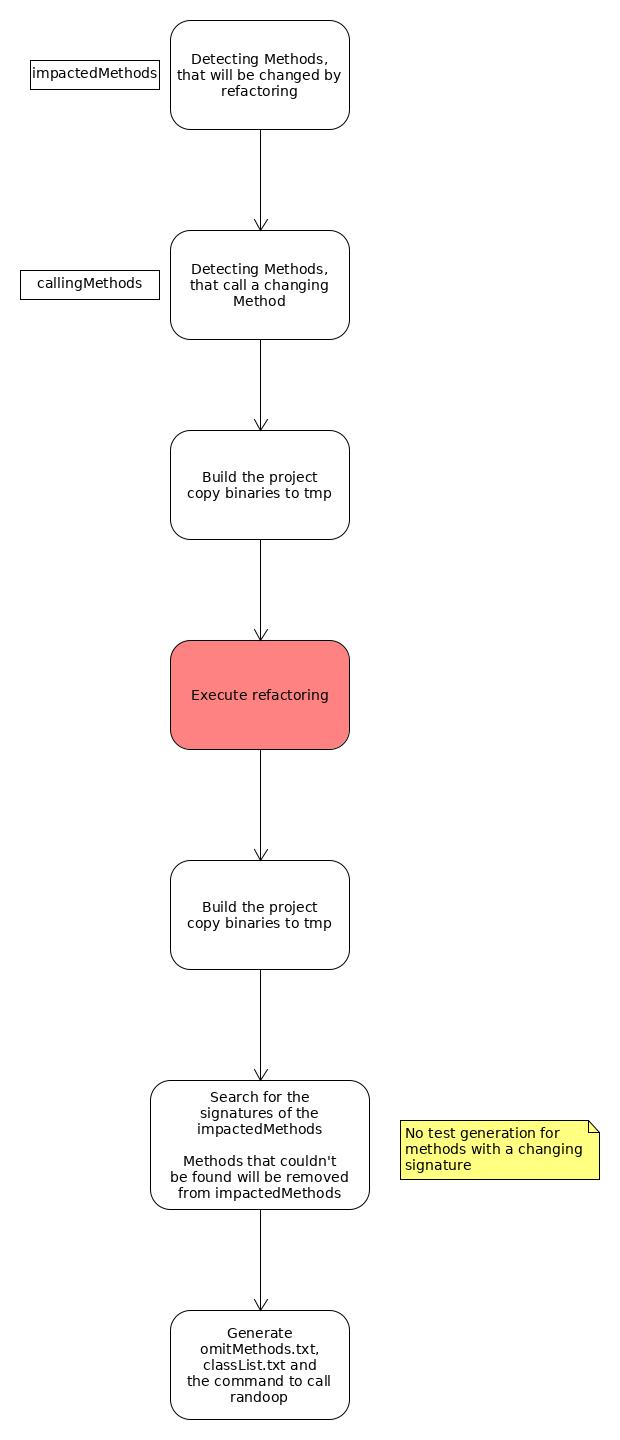
\includegraphics[height=\textheight-100pt]{Ablaufdiagramm.jpg}
	\chapter{Code location}
		Our code is located in the following three packages:
		\begin{itemize}
			\item \textit{\textbf{de.tudarmstadt.rxrefactoring.core.internal.execution.ipl}}\\
				Main Part of our code: The JavaVisitor traverses Eclipse ASTs. The MethodScanner searches for impacted and calling methods. The Randoop Generator builds the project, copies the binaries and calls Randoop.
			\item \textit{\textbf{de.tudarmstadt.rxrefactoring.core.internal.execution.ipl.collect}}\\
				Collections we needed, basically a Pair Class.
			\item \textit{\textbf{de.tudarmstadt.rxrefactoring.core.internal.execution.ipl.filter}}\\
				FilteredArrayList which is used in the JavaVisitor to collect the nodes, that match a given Filter.
		\end{itemize}
		Furthermore we added some code to \textit{de.tudarmstadt.rxrefactoring.core.internal.execution.RefactorExecution}, to obtain the ASTs, before and after refactoring. Everything that has to be executed before refactoring is added to \textit{doRefactorProject(...)}. Everything that has to be executed after the OK-Button has been clicked is added to \textit{run()}. 
		
		All changes in \textit{RefactorExecution} are marked with an inline comment beginning with "IPL".
\end{document}